\documentclass[10pt,journal,compsoc]{IEEEtran}
\usepackage{enumerate}
\usepackage{cite}
\usepackage{amsmath}
\interdisplaylinepenalty=2500
\usepackage{algorithm}
\usepackage{algorithmic}
\usepackage{graphicx}
\usepackage{multirow}
\usepackage{subfigure}
\usepackage{amssymb}
\usepackage[normalem]{ulem}
\usepackage{color}
\hyphenation{op-tical net-works semi-conduc-tor}
\newcommand{\rmnum}[1]{\expandafter{\romannumeral #1\relax}}

\begin{document}

\title{Dynamic Random Testing of Web Services: \\ A Methodology and Evaluation}


\author{Chang-ai~Sun,~\IEEEmembership{Senior Member,~IEEE,}
        Hepeng~Dai,
        Guan~Wang,
        Dave~Towey,~\IEEEmembership{Member,~IEEE,}
        Kai-Yuan~Cai,~\IEEEmembership{Member,~IEEE,}
        and~Tsong Yueh~Chen,~\IEEEmembership{Member,~IEEE,}
\thanks{A preliminary version of this paper was presented at the 36th Annual IEEE Computer Software and Applications Conference (COMPSAC 2012)~\cite{sun2012towards}.}
\thanks{C.-A. Sun, H. Dai, and G. Wang are with the School of Computer and Communication Engineering, University of Science and Technology Beijing, Beijing 100083, China. E-mail: casun@ustb.edu.cn.}% <-this % stops a space
\thanks{D. Towey is with the School of Computer Science, University of Nottingham Ningbo China, Ningbo 315100, China. E-mail: dave.towey@nottingham.edu.cn}
\thanks{K.-Y. Cai is with the School of Automation Science and Electrical Engineering, Beihang University, Beijing 100191, China. E-mail: kycai@buaa.edu.cn.}% <-this % stops a
\thanks{T.Y. Chen is with the Department of Computer Science and Software Engineering, Swinburne University of Technology, Hawthorn VIC 3122, Australia. Email: tychen@swin.edu.au.}
}


\markboth{IEEE TRANSACTIONS ON SERVICES COMPUTING,~submitted}%
{Sun \MakeLowercase{\textit{Sun et al.}}: An Empirical Study on Dynamic Random Testing of Web Services: A Methodology and Evaluation}


\IEEEtitleabstractindextext{
\begin{abstract}
  In recent years, Service Oriented Architecture (SOA) has been increasingly adopted to develop distributed applications in the context of the Internet. To develop reliable SOA-based applications, an important issue is how to ensure the quality of web services. In this paper, we propose a dynamic random testing (DRT) technique for web services, which is an improvement over the widely-practiced random testing (RT)~and partition testing (PT). We examine key issues when adapting DRT to the context of SOA, including a framework, guidelines for parameter settings, and a prototype for such an adaptation. Empirical studies are reported where DRT is used to test three real-life web services, and mutation analysis is employed to measure the effectiveness. Our experimental results show that, compared with the two baseline techniques, RT and Random Partition Testing (RPT), DRT demonstrates higher fault-detection effectiveness with a lower test case selection overhead. Furthermore, the theoretical guidelines of parameter setting for DRT are confirmed to be effective. The proposed DRT and the prototype provide an effective and efficient approach for testing web services.
\end{abstract}

\begin{IEEEkeywords}
Software Testing, Random Testing, Dynamic Random Testing, Web Service, Service Oriented Architecture.
\end{IEEEkeywords}}

\maketitle

\IEEEdisplaynontitleabstractindextext


\IEEEpeerreviewmaketitle


\section{Introduction}
\label{sec:introduction}

\IEEEPARstart{T}{est} result verification is an important part of software testing. A test oracle \cite{weyuker1982testing} is a mechanism that can exactly decide whether the output produced by a programs is correct. However, there are situations where it is difficult to decide whether the result of the software under test (SUT) agrees with the expected result. This situation is known as oracle problem \cite{barr2015oracle, patel2018mapping}. In order to alleviate the oracle problem, several techniques have been proposed, such as N-version testing \cite{brilliant1990performance}, metamorphic testing (MT) \cite{chen1998metamorphic, chen2018metamorphic}, assertions \cite{sim2014eliminating}, and machine learning \cite{chan2009pat}. Among of them, MT obtains metamorphic relations (MRs) according to the properties of SUT. Then, MRs are used to generate new test cases called follow-up test cases from original test cases known as source test cases. Next, both source and follow-up test cases are executed and their result are verified against the corresponding MRs.

The fault-detecting efficiency of MT relies on the quality of MRs and the source test cases. There are astronomically large number of studies to investigate generate good MRs \cite{chen2004case, cao2013correlation, sun2011metamorphic, chen2014metric, xie2016looking} or the source test cases \cite{chen2004metamorphic, batra2011efficient, dong2013security}. However, Researchers ignore the impact of test execution on the efficiency of MT. Random testing (RT) that randomly selects test cases from input domain (which refers to the set of all possible inputs of SUT), which is most
commonly used technique in traditional MT \cite{segura2016survey}. Although RT is simple to implement, RT does not make use of any execution information about SUT or the test history. Thus, traditional MT may be inefficient in some situations.

In contrast to RT, partition testing (PT) attempts to generate test cases in a more systematic way, aiming to use fewer test cases to detect more faults. When conducting PT, the input domain of SUT is divided into disjoint partitions, with test cases then selected from each and every one. Each partition is expected to have a certain degree of homogeneity, that is, test cases in the same partition should have similar software execution behavior: If one input can detect a fault, then all other inputs in the same partition should also be able to detect a fault. RT and PT have their own characteristics. Therefore, it is a nature thought to investigate the integration of them for developing new testing techniques. Sun et al. \cite{sun2018adaptive} proposed adaptive partition testing (APT) that takes advantages of testing information to control the testing process, with the goal of benefitting from the advantages of RT and PT.

In this study, we investigate how to make use of feedback information in the previous tests to control the execution process of MT. As a result, an adaptive metamorphic testing framework is proposed to improve the fault-detecting efficiency of MT. An empirical study was conducted to evaluate the efficiency of the proposed technique. Main contributions made in this paper are the following:





The rest of this paper is organized as follows.
Section~\ref{sec:background} introduces the underlying concepts for DRT, web services and mutation analysis.
Section~\ref{sec:DRTforwebserivce} presents the DRT framework for web services, guidelines for its parameter settings, and a prototype that partially automates DRT.
Section~\ref{sec:empiricalstudy} describes an empirical study where the proposed DRT is used to test three real-life web services, the results of which are summarized in Section~\ref{sec:results}.
Section~\ref{sec:relatedwork} discusses related work and Section~\ref{sec:conclusion} concludes the paper.

\section{Background}
\label{sec:background}

In this section, we present some of the underlying concepts for DRT, web services, and mutation analysis.

\subsection{Metamorphic Testing (MT)}

\label{section:mt}

MT is a novel technique to alleviate the oracle problem: Instead of applying an oracle, MT uses a set of MRs (corresponding to some specific properties of the SUT) to verify the test results. MT is normally conducted according to the following steps:

\begin{description}
  \item [Step1.]
  Identify an MR from the specification of the SUT.
  \item [Step2.]
  Generate the source test case $stc$ using the traditional test cases generation techniques.
  \item [Step3.]
  Derive the follow-up test case $ftc$ from the $stc$ based on the MR.
  \item [Step3.]
  execute $stc$ and $ftc$ and get their outputs $O_s$ and $O_f$.
  \item [Step4.]
  Verify $stc$, $ftc$, $O_s$, and $O_f$ against the MR: If the MR does not hold, a fault is said to be detected.
\end{description}
The above steps can be repeated for a set of MRs.

Let us use a simple example to illustrate how MT works. For instance, consider the mathematic function $f(x,y)$ that can calculate the maximal value of two integers $x$ and $y$. There is a simple yet obvious property: the order of two parameters $x$ and $y$ does not affect the output, which can be described as the follow metamorphic relation (MR): $f(x,y) = f(y,x)$. In this MR, $(x,y)$ is source test case, and $(y,x)$ is considered as follow-up test case. Suppose \texttt{P} denotes a program that implements the function $f(x,y)$, \texttt{P} is executed with a test cases $(1,2)$ and $(2,1)$. Then we check $P(1,2) = P(2,1)$: If the equality does not hold, then we consider that \texttt{P} at least has one fault.

\subsection{Adaptive Partition Testing (APT)}
\label{sec:apt}

DRT combines RT and PT [31], with the goal of benefitting from the advantages of both.
Given a test suite \emph{TS} classified into $m$ partitions (denoted $s_1, s_2, \ldots, s_m$),  suppose that a test case from $s_i$ ($i = 1, 2, \ldots, m$) is selected and executed.
If this test case reveals a fault, $\forall j = 1, 2, \ldots, m$ and $j \neq i$, we then set

\begin{equation}
\label{eq:DRThitJ}
p'_j =
\begin{cases}
p_j - \displaystyle\frac{\varepsilon}{m-1} & \text{if } p_j \geq \displaystyle\frac{\varepsilon}{m-1} \\
0 & \text{if } p_j < \displaystyle\frac{\varepsilon}{m-1}
\end{cases},
\end{equation}
where $\varepsilon$ is a probability adjusting factor, and then

\begin{equation}
\label{eq:DRThitI}
  p'_i = 1 - \sum_{\substack{j = 1 \\ j \neq i}}^m p'_j.
\end{equation}

Alternatively, if the test case does not reveal a fault, we set

\begin{equation}
\label{eq:DRTmissI}
p'_i =
\begin{cases}
p_i - \varepsilon & \text{if } p_i \geq \varepsilon \\
0 & \text{if } p_i < \varepsilon
\end{cases},
\end{equation}

and then for $\forall j = 1, 2, \ldots, m$ and $j \neq i$, we set

\begin{equation}
\label{eq:DRTmissJ}
p'_j =
\begin{cases}
p_j + \displaystyle\frac{\varepsilon}{m-1} & \text{if } p_i \geq \varepsilon \\
p_j + \displaystyle\frac{p'_i}{m-1} & \text{if } p_i < \varepsilon
\end{cases}.
\end{equation}

Algorithm \ref{alg:DRT} describes DRT.
In DRT, the first test case is taken from a partition that has been randomly selected according to the initial probability profile $\{p_1, p_2, \ldots, p_m\}$ (Lines 2 and 3 in Algorithm~\ref{alg:DRT}).
After each test case execution, the testing profile $\{ \left \langle s_1,p_1 \right \rangle, \left \langle s_2,p_2 \right \rangle, \ldots, \left \langle s_m,p_m \right \rangle\}$ is updated by changing the values of $p_i$:
If a fault is revealed, Formulas~\ref{eq:DRThitJ} and~\ref{eq:DRThitI} are used;
otherwise, Formulas~\ref{eq:DRTmissI} and~\ref{eq:DRTmissJ} are used.
The updated testing profile is then used to guide the random selection of the next test case (Line 8).
This process is repeated until a termination condition is satisfied (Line 1).
Examples of possible termination conditions include:
 ``testing resources have been exhausted'';
 ``a certain number of test cases have been executed''; and
 ``a certain number of faults have been detected".

\begin{algorithm}
    \caption{DRT}
    \label{alg:DRT}
    \begin{algorithmic}[1]
        \renewcommand{\algorithmicrequire}{\textbf{Input:}} %ʹ��ԭ���������ж��������\REQUIRE ��\ENSURE��ʾΪInput:��Output:
	    \renewcommand{\algorithmicensure}{\textbf{Output:}}
        \renewcommand{\algorithmicendwhile}{\algorithmicend\_\algorithmicwhile}
		\renewcommand{\algorithmicendfor}{\algorithmicend\_\algorithmicfor}
		\renewcommand{\algorithmicendif}{\algorithmicend\_\algorithmicif}
		\renewcommand{\algorithmicthen}{}
		\renewcommand{\algorithmicdo}{}
        \REQUIRE $\varepsilon, p_1, p_2, \ldots, p_m$
        \WHILE {termination condition is not satisfied}
        \STATE Select a partition $s_i$ according to the testing profile $\{ \left \langle s_1,p_1 \right \rangle, \left \langle s_2,p_2 \right \rangle, \ldots, \left \langle s_m,p_m \right \rangle\}$.
        \STATE Select a test case $t$ from $s_i$.
        \STATE Test the software using $t$.
        \IF {a fault is revealed by $t$}
        \STATE Update $p_j$ ($j = 1, 2, \ldots, m$ and $j \neq i$) and $p_i$ according to Formulas~\ref{eq:DRThitJ} and~\ref{eq:DRThitI}.
        \ELSE
        \STATE Update $p_j$ ($j = 1, 2, \ldots, m$ and $j \neq i$) and $p_i$ according to Formulas~\ref{eq:DRTmissI} and~\ref{eq:DRTmissJ}.
        \ENDIF
        \ENDWHILE
    \end{algorithmic}
\end{algorithm}

As can be seen from Formulas~\ref{eq:DRThitJ} to~\ref{eq:DRTmissJ},  updating the testing profile involves $m$ simple calculations, thus requiring a constant time.
Furthermore, the selection of partition $s_i$, and subsequent selection and execution of the test case, all involve a constant time.
The execution time for one iteration of DRT is thus a constant, and therefore the overall time complexity for DRT to select $n$ test cases is $O(m \cdot n)$.

\subsection{Adaptive Random Testing (ART)}
\label{section:art}





\section{SDMT}
\label{sec:sdmt}

In this section, we describe a framework for applying DRT to web services, discuss guidelines for DRT's parameter settings, and present a prototype that partially automates  DRT for web services.

\subsection{Motivation}
\label{sec:motavation}


\subsection{Framework}
\label{sec:framework}


\begin{figure}[]
  \centering
  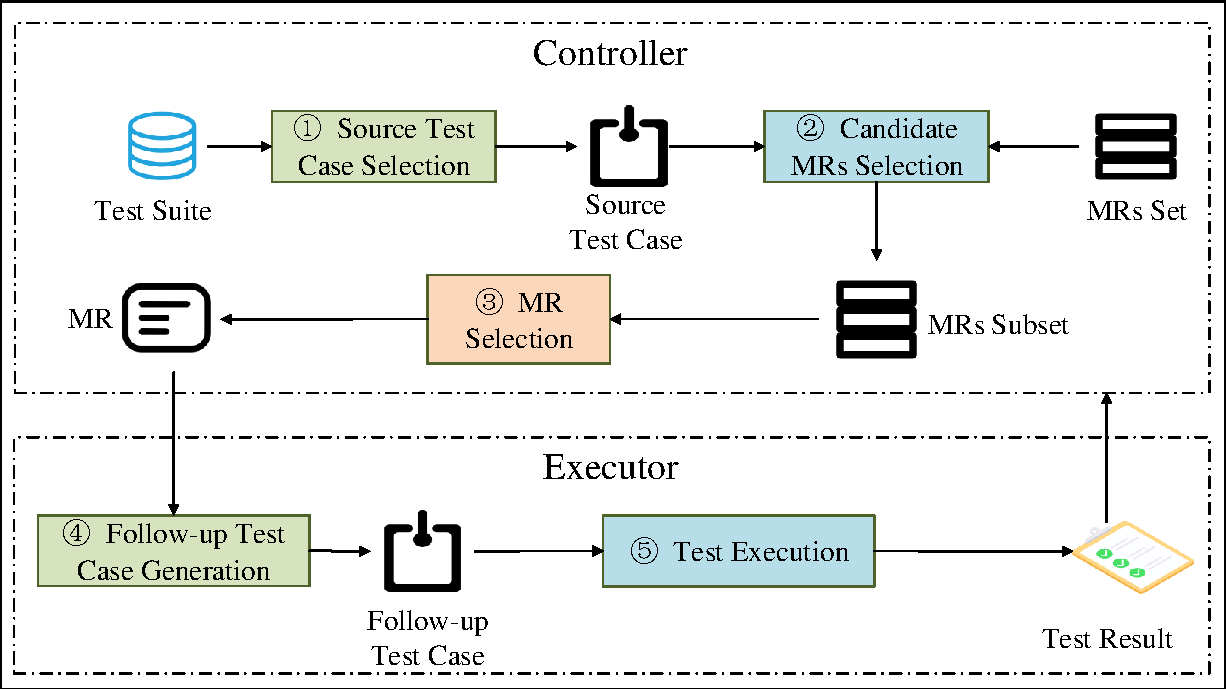
\includegraphics[width = 0.5\textwidth]{fig//generateframework}
  \caption{framework}
  \label{fig:framework}
\end{figure}

\begin{enumerate}[1]
  \item
  \emph{Source Test Case Selection}.
  
  \item
  \emph{candidate MRs Selection}.

  \item
  \emph{MR Selection}.

  \item
  \emph{Follow-up Test Case Generation}.

  \item
  \emph{Test Case Execution}.
  The relevant DRT component receives the generated test case, converts it into an input message, invokes the web service(s) through the SOAP protocol, and intercepts the test results (from the output message).
\end{enumerate}

\subsection{Updating Test Profile Strategies}
\label{sec:updatingTestProfile}

\subsection{Selecting MR Strategies}
\label{sec:selectingMR}

\subsection{Partition Based SDMT}
\label{sec:partitionSDMT}

\subsection{Random Based SDMT}
\label{sec:randomSDMT}

\section{Empirical Study}
\label{sec:empiricalStudy}

We conducted a series of empirical studies to evaluate the performance of DRT.

\subsection{Research Questions}
\label{sec:rqs}
In our experiments, we focused on addressing the following three research questions:
\begin{description}
  \item [\textbf{RQ1}] \textbf{How efficient is SDMT at detecting faults?}
  
  Fault-detection efficiency is a key criterion for evaluating the performance of a testing technique. In our study, we chose three real-life programs, and applied mutation analysis to evaluate the fault-detecting efficiency.
  
  \item [\textbf{RQ2}] \textbf{What is the actual test case selection overhead when using the M-AMT strategy?} 
  
  We evaluate the test case selection overhead of M-AMT and compare with traditional MT in detecting software faults.
\end{description}

\subsection{Object Programs}
\label{sec:programs}

In order to address our research questions, we chose to study four sets of object programs: three laboratorial programs that were developed according to corresponding specifications, seven programs from the Software-artifact Infrastructure Repository (SIR) \cite{do2005supporting}, the regular expression processor component of the larger utility program \texttt{GUN grep}, and a Java library developed by Alibaba, which can be used to convert Java Objects into their JSON representation, and convert a JSON string to an equivalent Java object. The details of twelve programs are summarized in Table \ref{table:objects}.
\begin{table*}[hbt]
  \caption{Twelve Programs as Experimental Objects}
  \label{table:objects}
  \centering
  \begin{tabular}{|c|c|c|c|c|c|c|c|} \hline
  programs               &Source        &Language  &LOC     &All Faults &Used Faults &Number of  &Number of  \\
                         &              &          &        &           &            &MRs        &Partitions\\ \hline
  \texttt{CUBS}          &Laboratory    &Java      &107     &187        &4           &184        &8 \\ \hline
  \texttt{ACMS}          &Laboratory    &Java      &128     &210        &9           &142        &4 \\ \hline      
  \texttt{ERS}           &Laboratory    &Java      &117     &180        &4           &1130       &12 \\ \hline
  \texttt{grep}          &GUN           &c         &10,068  &20         &20          &12         &-- \\ \hline
  \texttt{printtokens}   &SIR           &c         &483     &7          &7           &3          &-- \\ \hline
  \texttt{printtokens2}  &SIR           &c         &402     &10         &10          &3          &-- \\ \hline
  \texttt{replace}       &SIR           &c         &516     &31         &31          &3          &-- \\ \hline
  \texttt{schedule}      &SIR           &c         &299     &9          &9           &3          &-- \\ \hline
  \texttt{schedule2}     &SIR           &c         &297     &9          &9           &3          &-- \\ \hline
  \texttt{tcas}          &SIR           &c         &138     &41         &41          &3          &-- \\ \hline
  \texttt{totinfo}       &SIR           &c         &346     &23         &23          &3          &-- \\ \hline
  \texttt{FastJson}      &Alibaba       &Java      &204125  &6          &6           &--         &-- \\ \hline
  \end{tabular}
\end{table*}

There four sets of programs present complementary strengths and weaknesses as experiment objects. The Laboratorial programs implement simple functions and their interfaces are easy to understand. The test engineers can easily generate source test cases, and identify MRs for testing laboratorial programs. However, these programs are small and there are a limited number of faulty versions available for each programs. The SIR repositories provides object programs, including a number of pre-existing versions with seeded faults, as well as a test suite in which test cases were randomly generated. It is a challenge task to partition the input domain of those programs. The \texttt{grep} program is a much larger system for which mutation faults could be generated. The \texttt{FastJson} is also a much larger system, and the faults of that are obtained on GitHub.
We provide further details on each of those sets of object programs next.

\subsubsection{Laboratorial Programs}
\label{sec:labPrograms}

Based on three real-lift specifications, We developed three systems, respectively. \texttt{China Unicom Billing System (CUBS)} provides an interface through which customers can know how much they need to pay according to plans, month charge, calls, and data usage. The details of two cell-phone plans are summarized in Tables \ref{table:chinaA} and \ref{table:chinaB}. \texttt{Aviation Consignment Management System (ACMS)} aims to help airline companies check the allowance (weight) of free baggage, and the cost of additional baggage. Based on the destination, flights are categorized as either domestic or international. For international flights, the baggage allowance is greater if the passenger is a student (30kg), otherwise it is 20kg. Each aircraft offers three cabins classes from  which to choose (economy, business, and first), with passengers in different classes having different allowances. The detailed price rules are summarized in Table~\ref{table:acms}, where $price_0$ means economy class fare.
\texttt{Expense Reimbursement System (ERS)} assists the sales Supervisor of a company with handling the following tasks: \rmnum{1}) Calculating the cost of the employee who use the cars based on their titles and the number of miles actually traveled; \rmnum{2}) accepting the requests of reimbursement that include airfare, hotel accommodation, food and cell-phone expenses of the employee.

\begin{table}[!htp]
  \centering
  \caption{Plan A}
  \label{table:chinaA}
  \begin{tabular}{|c|c|c|c|c|c|} \hline
  \multicolumn{2}{|c|}{\multirow{2}{*}{Plan details}}  &\multicolumn{4}{|c|}{Month charge~(CNY)} \\ \cline{3-6}
  \multicolumn{2}{|c|}{}                                     &\!$option_1$\!  &\!$option_2$\!  &\!$option_3$\! &\!$option_4$\! \\ \hline
   \multirow{2}{*}{\rotatebox{90}{Basic}} &Free calls~(min)  &50  &96  &286 &3000   \\ \cline{2-6}
                                          &Free data~(MB)    &150 &240 &900 &3000\\ \hline
   \multirow{2}{*}{\rotatebox{90}{Extra}} &Dialing calls~(CNY/min)  &0.25 &0.15  &0.15 &0.15 \\ \cline{2-6}
                                          &Data~(CNY/KB)  &\multicolumn{4}{c|}{0.0003} \\ \hline
  \end{tabular}
\end{table}

\begin{table}[!htp]
  \caption{Plan B}
  \label{table:chinaB}
  \centering
  \begin{tabular}{|c|c|c|c|c|c|} \hline
  \multicolumn{2}{|c|}{\multirow{2}{*}{Plan details}}  &\multicolumn{4}{|c|}{Month charge~(CNY)} \\ \cline{3-6}
  \multicolumn{2}{|c|}{}                                     &\!$option_1$\!  &\!$option_2$\!  &\!$option_3$\! &\!$option_4$\! \\ \hline
   \multirow{2}{*}{\rotatebox{90}{Basic}} &Free calls~(min)  &120  &450  &680 &1180   \\ \cline{2-6}
                                          &Free data~(MB)    &40 &80 &100 &150\\ \hline
   \multirow{2}{*}{\rotatebox{90}{Extra}} &Dialing calls~(CNY/min)  &0.25 &0.15  &0.15 &0.15 \\ \cline{2-6}
                                          &Data~(CNY/KB)  &\multicolumn{4}{c|}{0.0003} \\ \hline
  \end{tabular}
\end{table}


\begin{table*}[!htp]
  \caption{ACMS Baggage Allowance and Pricing Rules}
  \label{table:acms}
  \centering
  \begin{tabular}{|c|c|c|c|c|c|c|} \hline
  \multirow{2}{*}{}     &\multicolumn{3}{c|}{Domestic flights}              &\multicolumn{3}{c|}{International flights} \\ \cline{2-7}
                                    &First class  &Business class   &Economy class   &First class  &Business class   &Economy class \\ \hline
  Carry~on (kg)                     &5       &5        &5        &7        &7        &7  \\ \hline
  Free checked-in (kg)              &40      &30       &20       &40       &30       &20/30 \\ \hline
  Additional baggage pricing~(kg)   &\multicolumn{3}{c|}{$price_0 * 1.5\%$}   &\multicolumn{3}{c|}{$price_0 * 1.5\%$}  \\ \hline
  \end{tabular}
\end{table*}

\subsubsection{SIR Programs}
\label{sec:SIRPrograms}

The seven object programs selected from the SIR [24] repository were \texttt{printtokens}, \texttt{printtokens2}, \texttt{replace}, \texttt{schedule}, \texttt{schedule2}, \texttt{tcas}, and \texttt{totinfo}. These programs were originally compiled by Hutchins et al. \cite{hutchins1994experiments} at Siemens Corporate Research. We used these programs for several reasons:
\begin{enumerate}[1]
  \item
  Faulty versions of the programs are available.
  
  \item
  The programs are of manageable size and complexity for an initial study.
  
  \item
  All programs and related materials are available from the SIR, and the MRs of each program are defined in  \cite{xie2013metamorphic}.
  
\end{enumerate}

The \texttt{printtokens} and \texttt{printtokens2} are independent implementations of the same specification. They each implement a lexical analyzer. Their input files are split into lexical tokens according to a tokenizing scheme, and their output is the separated tokens. The \texttt{replace} program is a command-line utility that takes a search string, a replacement string, and an input file. The search string is a regular expression. The replacement string is text, with some metacharacters to enable certain features. The \texttt{replace} program searches for occurrences of the search string in the input file, and produces an output file where each occurrence of the search string is replaced with the replacement string. The \texttt{schedule} and \texttt{schedule2} programs are also independent implementations of the same specification. They each implement a priority scheduler that takes three non-negative integers and an input file. The integers indicate the number of initial processes at the three available scheduling priorities. The \texttt{schedule} and \texttt{schedule2} programs then take as input a command file that specifies certain actions to be taken. The \texttt{tcas} program is a small part of a much larger aeronautical collision avoidance system. It performs simple analysis on data provided by other parts of the system and returns an integer indicating what action, if any, the pilot should take to avoid collision.

\subsubsection{GUN grep}
\label{sec:grep}

The used version of the \texttt{grep} programs is 2.5.1a \cite{grep}. This program searches one or more input files for lines containing a match to a specified pattern. By default, grep prints the matching lines. We chose \texttt{grep} for our study for several reasons:
\begin{enumerate}[1]
  \item
  The \texttt{grep} program is wide used in Unix system, providing a opportunity to demonstrate the real world relevance of our techniques.
  \item
  The \texttt{grep} program, and its input format, are of greater complexity than the the programs in the other test sets, but still manageable as a target for automated test case generation.
\end{enumerate}

The inputs of the \texttt{grep} were categorize into three components: options, which consist of a list of commands to modify the searching process, pattern, which is the regular expression to be searched for, and files, which refers to the input files to be searched.  

The scope of functionality of this program is larger, which leads to construct test infrastructure to test all of functionality would have been impractical. Therefore, we restricted our focus to the regular expression analyzer of \texttt{grep}.

\subsubsection{Real-World Popular Programs}
\label{sec:realPragrams}
The \texttt{FastJson} 


\subsection{Variables}

\subsubsection{Independent Variables}

The independent variable is the testing technique, DRT. RPT and RT were used as baseline techniques for comparison.

\subsubsection{Dependent Variables}

The dependent variable for RQ1 is the metric for evaluating the fault-detection effectiveness.
Several effectiveness metrics exist, including:
the P-measure~\cite{duran1984evaluation} (the probability of at least one fault being detected by a test suite);
the E-measure~\cite{chen1997optimal} (the expected number of faults detected by a test suite);
the F-measure~\cite{sun2018adaptive} (the expected number of test case executions required to detect the first fault); and
the T-measure~\cite{zhang2014history} (the expected number of test cases required to detect all faults).
Since the F- and T-measures have been widely used for evaluating the fault-detection efficiency and effectiveness of DRT-related testing techniques~\cite{Cai07, cai2009random, Lv2011, Yang2014Dynamic, li2015, zhang2014history}, they are also adopted in this study.
We use $F$ and $T$ to represent the F-measure and the T-measure of a testing method.
As shown in Algorithm~\ref{alg:DRT}, the testing process may not terminate after the detection of the first fault.
Furthermore, because the fault detection information can lead to different probability profile adjustment mechanisms, it is also important to see what would happen after revealing the first fault.
Therefore, we introduce the F2-measure~\cite{sun2018adaptive} as is the number of additional test cases required to reveal the second fault after detection of the first fault.
We use $F2$ to represent the F2-measure of a testing method, and $SD_{measure}$ to represent the standard deviation of metrics (where $measure$ can be $F$, $F2$, or $T$).

An obvious metric for RQ3 is the time required to detect faults.
Corresponding to the T-measure, in this study we used $T$-$time$, the time required to detect all faults.
$F$-$time$ and $F2$-$time$ denote the time required to detect the first fault, and the additional time needed to detect the second fault (after detecting the first), respectively.
For each of these metrics, smaller values indicate a better performance.

\subsection{Experimental Settings}

\subsubsection{Partitioning}



\subsubsection{Initial Test Profile}


\subsubsection{Constants}


\subsection{Experimental Environment}
\subsection{Experiment Architecture}


\subsection{Threats To Validity}

\subsubsection{Internal Validity}


\subsubsection{External Validity}



\subsubsection{Construct Validity}


\subsubsection{Conclusion Validity}




\section{Experimental Results}
\label{sec:results}



\section{Related Work}
\label{sec:relatedwork}

In this section, we describe related work from two perspectives:
related to testing techniques for web services; and
related to improving RT and PT.


\section*{Acknowledgment}

This research is supported by
the National Natural Science Foundation of China (Grant Nos. 61872039 and 61872167),
the Beijing Natural Science Foundation (Grant No. 4162040),
the Aeronautical Science Foundation of China (Grant No. 2016ZD74004), and
the Fundamental Research Funds for the Central Universities (Grant No. FRF-GF-17-B29).
\ifCLASSOPTIONcaptionsoff
  \newpage
\fi
\bibliographystyle{IEEEtran}
\bibliography{MT}
\vspace{-10ex}
\begin{IEEEbiography}[{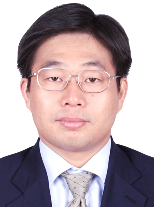
\includegraphics[width=1in,height=1.25in,clip,keepaspectratio]{fig/authors/CASun.pdf}}]{Chang-ai Sun} is a Professor in the School of Computer and Communication Engineering, University of Science and Technology Beijing.
Before that, he was an Assistant Professor at Beijing Jiaotong University, China, a postdoctoral fellow at the Swinburne University of Technology, Australia, and a postdoctoral fellow at the University of Groningen, The Netherlands. He received the bachelor degree in Computer Science from the University of Science and Technology Beijing, China, and the PhD degree in Computer Science from Beihang University, China.
His research interests include software testing, program analysis, and Service-Oriented Computing.
\end{IEEEbiography}
\vspace{-10ex}
\begin{IEEEbiography}[{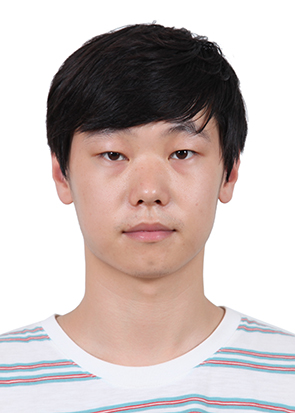
\includegraphics[width=1in,height=1.25in,clip,keepaspectratio]{fig/authors/HPDai.jpg}}]{Hepeng Dai} is a PhD student in the School of Computer and Communication Engineering, University of Science and Technology Beijing, China. He received the master degree in Software Engineering from University of Science and Technology Beijing, China and the bachelor degree in Information and Computing Sciences from China University of Mining and Technology, China. His current research interests include software testing and debugging.
\end{IEEEbiography}
\vspace{-10ex}
\begin{IEEEbiography}[{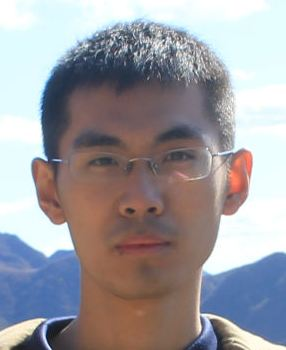
\includegraphics[width=1in,height=1.25in,clip,keepaspectratio]{fig/authors/GWang.jpg}}]{Guan Wang} is a masters student at the School of Computer and Communication Engineering, University of Science and Technology Beijing. He received a bachelor degree in Computer Science from University of Science and Technology Beijing. His current research interests include software testing and Service-Oriented Computing.
\end{IEEEbiography}
\vspace{-10ex}
\begin{IEEEbiography}[{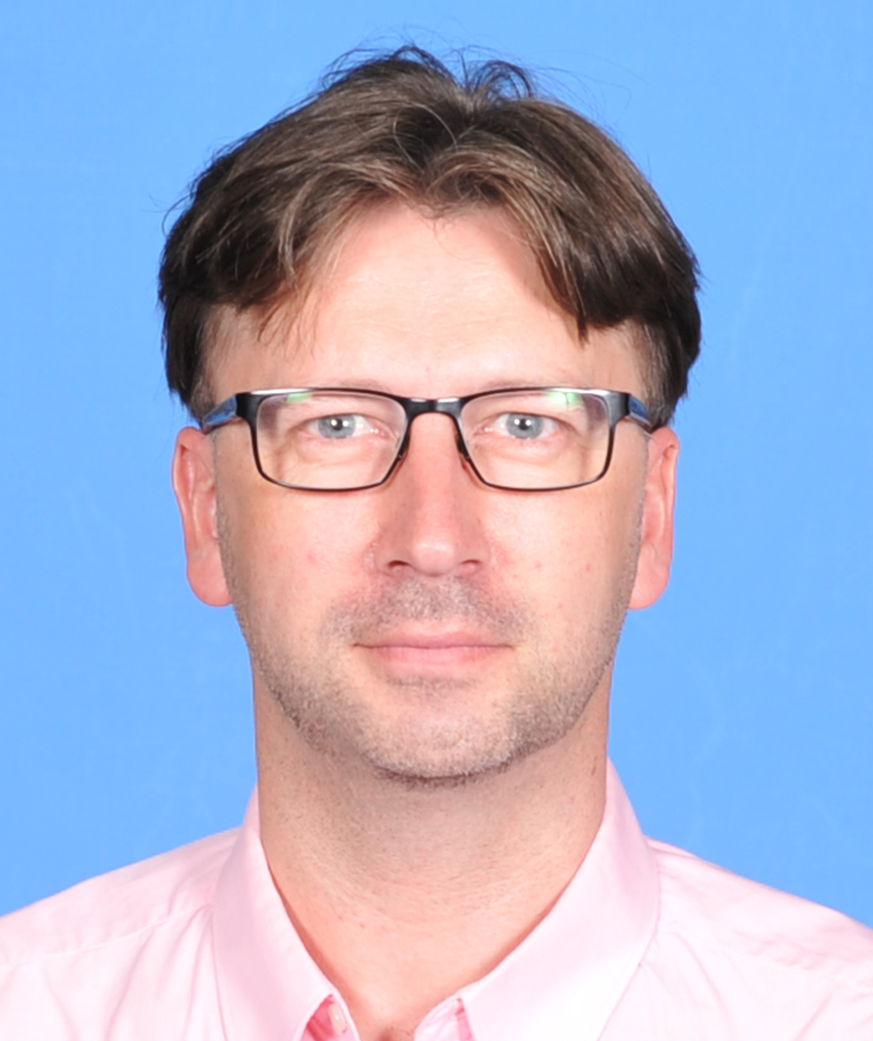
\includegraphics[width=1in,height=1.25in,clip,keepaspectratio]{fig/authors/DaveTowey.png}}]{Dave Towey} is an associate professor in the School of Computer Science, University of Nottingham Ningbo China. He received his BA and MA degrees from The University of Dublin, Trinity College, PgCertTESOL from The Open University of Hong Kong, MEd from The University of Bristol, and PhD from The University of Hong Kong. His current research interests include technology-enhanced teaching and learning, and software testing, especially metamorphic testing and adaptive random testing. He is a  member of both the IEEE and the ACM.
\end{IEEEbiography}
\vspace{-10ex}
\begin{IEEEbiography}[{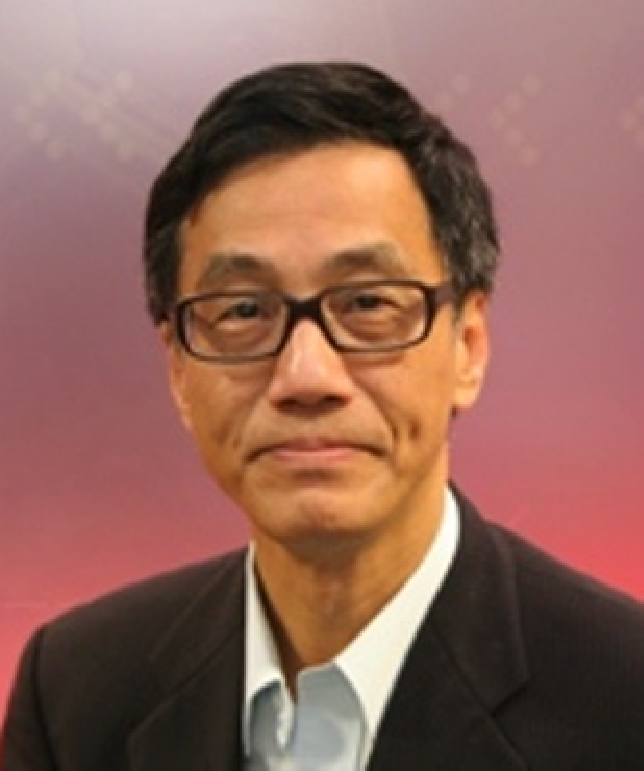
\includegraphics[width=1in,height=1.25in,clip,keepaspectratio]{fig/authors/TYChen.pdf}}]{Tsong Yueh Chen} is a Professor of Software Engineering at the Department of Computer Science and Software Engineering in Swinburne University of Technology. He received his PhD in Computer Science from The University of Melbourne, the MSc and DIC from Imperial College of Science and Technology, and BSc and MPhil from The University of Hong Kong. He is the inventor of metamorphic testing and adaptive random testing.
\end{IEEEbiography}
\vspace{-10ex}
\begin{IEEEbiography}[{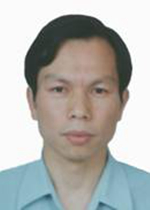
\includegraphics[width=1in,height=1.25in,clip,keepaspectratio]{fig/authors/KYCai.pdf}}]{Kai-Yuan Cai} received the BS, MS, and PhD degrees from Beihang university, Beijing, China, in 1984, 1987, and 1991, respectively. He has been a full professor at Beihang University since 1995. He is a Cheung Kong Scholar (chair professor), jointly appointed by the Ministry of Education of China and the Li Ka Shing Foundation of Hong Kong in 1999. His main research interests include software testing, software reliability, reliable flight control, and software cybernatics.
\end{IEEEbiography}

\end{document}
